\documentclass[12pt,letterpaper]{article}

\usepackage[utf8]{inputenc}
\usepackage[T1]{fontenc}
\usepackage[spanish]{babel}
\usepackage{geometry}
\usepackage{graphicx}
\usepackage{float}
\usepackage{booktabs}
\usepackage{array}
\usepackage{longtable}
\usepackage{hyperref}
\usepackage{amsmath}
\usepackage{enumitem}
\usepackage{xcolor}
\usepackage{caption}

\geometry{margin=2.5cm}
\graphicspath{{outputs_lab03/figures/}{figures/}}
\hypersetup{colorlinks=true, linkcolor=black, urlcolor=blue, citecolor=black}
\setlist[itemize]{leftmargin=*}
\setlist[enumerate]{leftmargin=*}

\title{\textbf{Estudio de Caso sobre Métodos de Aprendizaje Supervisado para Regresión}\\
Análisis, Modelado y Evaluación de Técnicas de Regresión}
\author{David Núñez Franco \\ Angel Leiva Abarca \\ Billy Cordero Porras}
\date{Mayo 2026}

\begin{document}
\maketitle

\begin{abstract}
Los métodos supervisados de regresión permiten construir modelos predictivos cuando la variable de respuesta es cuantitativa. En este laboratorio se desarrolla un estudio de caso utilizando el conjunto de datos Diabetes, con el objetivo de comparar distintos algoritmos de regresión: regresión lineal, regresión penalizada con Ridge y Lasso, KNN, árboles de regresión, Random Forest, SVR y métodos de potenciación como AdaBoost, Gradient Boosting y XGBoost. El análisis integra preprocesamiento, imputación, escalamiento, selección de atributos, validación cruzada, evaluación en prueba y visualización de residuos. Los resultados muestran que los modelos lineales y penalizados presentan el mejor equilibrio en validación cruzada, mientras que algunos modelos no lineales mejoran métricas puntuales en el conjunto de prueba. 
\end{abstract}

\textbf{Palabras clave:} aprendizaje supervisado, regresión, Ridge, Lasso, KNN, SVR, Random Forest, AdaBoost, XGBoost.

\section{Introducción}
El aprendizaje supervisado se fundamenta en conjuntos de datos donde cada observación contiene variables predictoras y una variable de respuesta conocida. Cuando la variable objetivo es continua, el problema se clasifica como regresión. A diferencia de la clasificación, donde el modelo asigna una clase discreta, en regresión se estima un valor numérico.

Este laboratorio mantiene la estructura metodológica de los laboratorios previos: primero se estudian los fundamentos conceptuales de los algoritmos, luego se prepara el conjunto de datos, se definen configuraciones estándar y variaciones, se ejecuta un benchmark comparativo y finalmente se selecciona e interpreta el mejor modelo.

\section{Descripción del conjunto de datos}
El estudio se desarrolló con el conjunto de datos Diabetes de \texttt{scikit-learn}, utilizado como problema clásico de regresión. El dataset contiene 442 observaciones y 10 variables predictoras cuantitativas. La variable objetivo, llamada \texttt{target}, representa una medida cuantitativa de progresión de la enfermedad.

\begin{table}[H]
\centering
\caption{Características generales del dataset Diabetes.}
\begin{tabular}{lr}
\toprule
Característica & Valor \\
\midrule
Observaciones & 442 \\
Variables predictoras & 10 \\
Variables totales & 11 \\
Valores faltantes & 0 \\
Variable objetivo & \texttt{target} \\
Tipo de problema & Regresión \\
Mínimo del objetivo & 25.00 \\
Máximo del objetivo & 346.00 \\
Media del objetivo & 152.13 \\
Desviación estándar del objetivo & 77.09 \\
\bottomrule
\end{tabular}
\end{table}

El dataset es adecuado para regresión porque la variable de respuesta es numérica continua y las variables predictoras son cuantitativas. La Figura \ref{fig:dist_target} muestra la distribución de la variable objetivo.

\begin{figure}[H]
\centering
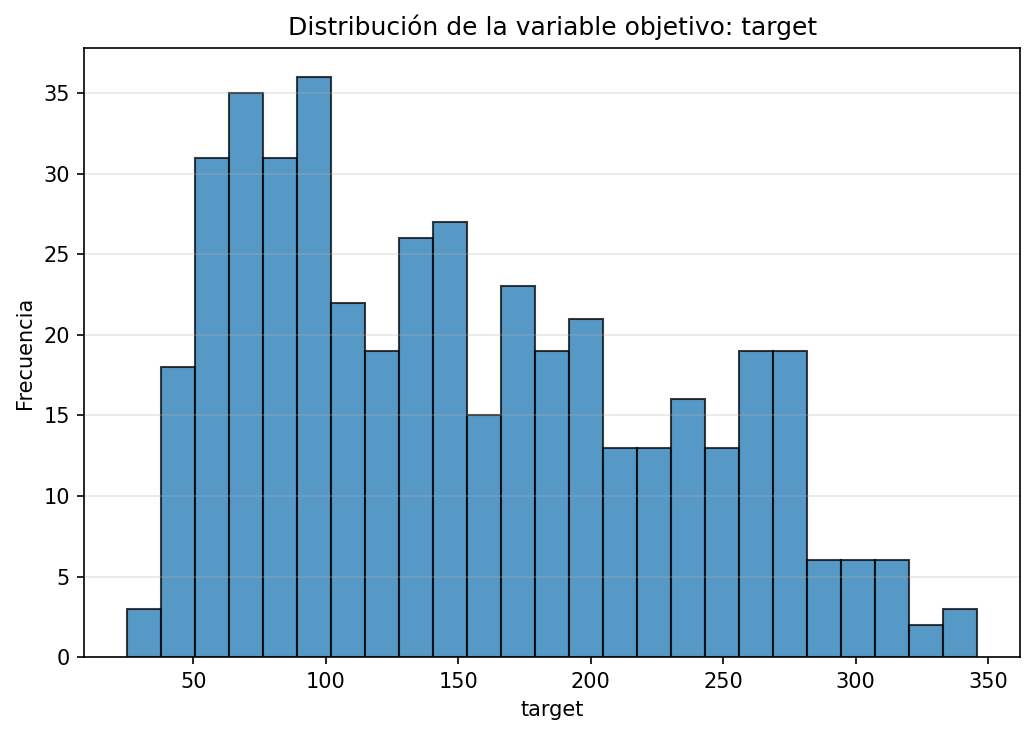
\includegraphics[width=0.75\textwidth]{distribucion_target.png}
\caption{Distribución de la variable objetivo del dataset Diabetes.}
\label{fig:dist_target}
\end{figure}

\begin{figure}[H]
\centering
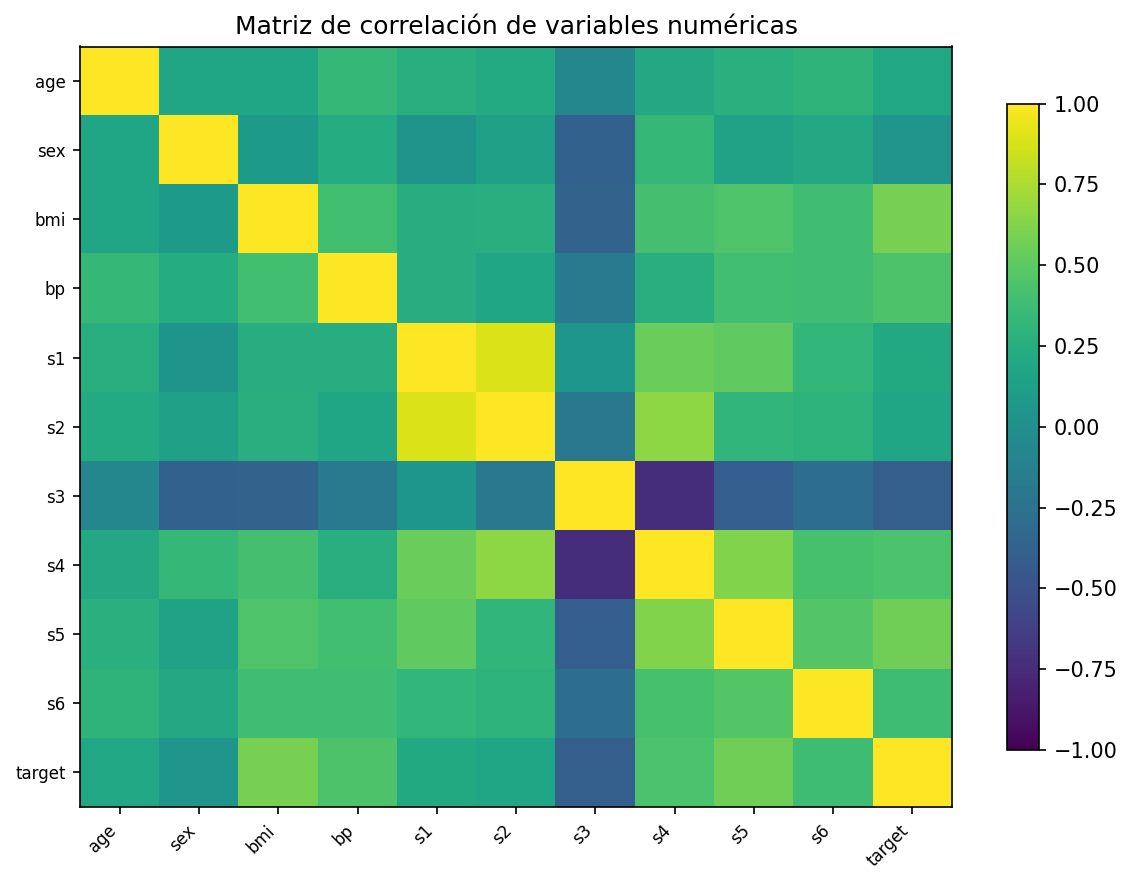
\includegraphics[width=0.85\textwidth]{correlacion_numericas.png}
\caption{Matriz de correlación de las variables numéricas.}
\label{fig:corr}
\end{figure}

\section{Fundamentos teóricos de los algoritmos}

\subsection{Regresión lineal simple y múltiple}
La regresión lineal modela la relación entre una variable dependiente continua y una o más variables independientes. En su forma múltiple, el modelo se expresa como:
\begin{equation}
\hat{y}=\beta_0 + \beta_1x_1 + \beta_2x_2 + \cdots + \beta_px_p.
\end{equation}
El ajuste se obtiene minimizando la suma de errores cuadráticos entre los valores reales y predichos. Su principal ventaja es la interpretabilidad de los coeficientes; sin embargo, puede ser sensible a multicolinealidad, valores atípicos y relaciones no lineales.

\subsection{Regresión penalizada Ridge}
Ridge incorpora una penalización $L_2$ sobre los coeficientes del modelo lineal:
\begin{equation}
\min_{\beta} \sum_{i=1}^{n}(y_i-\hat{y}_i)^2 + \lambda\sum_{j=1}^{p}\beta_j^2.
\end{equation}
La penalización reduce la magnitud de los coeficientes y ayuda a controlar la varianza del modelo, especialmente cuando existen variables correlacionadas.

\subsection{Regresión penalizada Lasso}
Lasso utiliza una penalización $L_1$:
\begin{equation}
\min_{\beta} \sum_{i=1}^{n}(y_i-\hat{y}_i)^2 + \lambda\sum_{j=1}^{p}|\beta_j|.
\end{equation}
A diferencia de Ridge, Lasso puede llevar algunos coeficientes exactamente a cero, por lo que también funciona como método de selección automática de variables.

\subsection{KNN para regresión}
KNN para regresión estima el valor de una nueva observación promediando los valores de respuesta de sus $k$ vecinos más cercanos. Su rendimiento depende de la métrica de distancia, del valor de $k$ y del escalamiento de las variables. En este laboratorio se usa \texttt{StandardScaler} para evitar que variables con mayor escala dominen el cálculo de distancia.

\subsection{Árboles de regresión}
Los árboles de regresión dividen recursivamente el espacio de predictores mediante reglas del tipo ``si-entonces''. En cada nodo se busca una partición que reduzca la variabilidad de la variable objetivo. Su ventaja principal es la interpretabilidad, aunque árboles muy profundos pueden sobreajustarse.

\subsection{Random Forest para regresión}
Random Forest es un ensamble de árboles de decisión. Cada árbol se entrena sobre una muestra bootstrap y, en cada división, se considera un subconjunto aleatorio de variables. Para regresión, la predicción final se obtiene promediando las predicciones individuales. Este enfoque reduce la varianza de un árbol individual y mejora la robustez.

\subsection{Máquinas de Soporte Vectorial para Regresión}
SVR busca una función que aproxime los datos dentro de un margen de tolerancia $\epsilon$. Mediante kernels puede modelar relaciones no lineales. Requiere escalamiento de variables y una adecuada selección de parámetros como $C$, $\epsilon$ y \texttt{gamma}.

\subsection{AdaBoost y XGBoost para regresión}
AdaBoost y XGBoost pertenecen a la familia de \textit{boosting}. AdaBoost ajusta modelos secuenciales dando más peso a observaciones difíciles, mientras que XGBoost construye árboles aditivos que corrigen gradientes de una función de pérdida e incorpora regularización. Aunque en algunos enunciados se menciona ``bootstrap'', técnicamente AdaBoost y XGBoost corresponden a potenciación o \textit{boosting}; el uso explícito de bootstrap es más característico de Random Forest.

\section{Metodología experimental}

\subsection{Preprocesamiento}
El flujo de preparación incluyó:
\begin{enumerate}
    \item Carga del dataset Diabetes.
    \item Separación entre variables predictoras y variable objetivo.
    \item Validación de que la variable objetivo fuera cuantitativa.
    \item Imputación por mediana para variables numéricas.
    \item Codificación one-hot para variables categóricas, si existieran.
    \item Escalamiento opcional con \texttt{StandardScaler}, \texttt{MinMaxScaler} o \texttt{RobustScaler} según el algoritmo.
    \item Selección opcional de atributos mediante \texttt{SelectKBest} con \texttt{f\_regression}.
    \item Partición 75\% entrenamiento y 25\% prueba con semilla fija.
\end{enumerate}

\subsection{Modelos evaluados}
Se evaluaron configuraciones estándar y variaciones para los siguientes algoritmos:
\begin{itemize}
    \item \texttt{LinearRegression}
    \item \texttt{Ridge} y \texttt{RidgeCV}
    \item \texttt{Lasso} y \texttt{LassoCV}
    \item \texttt{KNeighborsRegressor}
    \item \texttt{SVR}
    \item \texttt{DecisionTreeRegressor}
    \item \texttt{RandomForestRegressor}
    \item \texttt{AdaBoostRegressor}
    \item \texttt{GradientBoostingRegressor}
    \item \texttt{XGBRegressor}, cuando está disponible el paquete \texttt{xgboost}
\end{itemize}

\subsection{Métricas de evaluación}
Las métricas utilizadas fueron:
\begin{itemize}
    \item \textbf{RMSE}: raíz del error cuadrático medio. Penaliza errores grandes y se usa como criterio principal.
    \item \textbf{MAE}: error absoluto medio. Mide el error promedio en las mismas unidades del objetivo.
    \item \textbf{$R^2$}: proporción de variabilidad explicada por el modelo.
    \item \textbf{MAPE}: error porcentual absoluto medio.
\end{itemize}

La selección automática del mejor modelo se realizó priorizando menor RMSE promedio en validación cruzada, luego menor RMSE en prueba y, como desempate, mayor $R^2$.

\section{Resultados experimentales}

\subsection{Benchmark general}
La Tabla \ref{tab:benchmark} muestra las diez mejores configuraciones ordenadas por RMSE de validación cruzada.

\begin{table}[H]
\centering
\caption{Benchmark de modelos de regresión.}
\label{tab:benchmark}
\resizebox{\textwidth}{!}{%
\begin{tabular}{llllll}
\toprule
Modelo & Algoritmo & CV RMSE & CV $R^2$ & Test RMSE & Test $R^2$ \\
\midrule
Regresion\_Lineal & LinearRegression & 55.6310 & 0.4815 & 53.3696 & 0.4849 \\
Lasso\_alpha\_0\_01 & Lasso & 55.6336 & 0.4815 & 53.3590 & 0.4851 \\
Ridge\_alpha\_1 & Ridge & 55.6629 & 0.4809 & 53.3182 & 0.4859 \\
RidgeCV & RidgeCV & 55.8193 & 0.4781 & 53.3070 & 0.4861 \\
LassoCV & LassoCV & 55.9651 & 0.4752 & 53.2768 & 0.4867 \\
Regresion\_Lineal\_SelectK & LinearRegression & 56.8691 & 0.4573 & 53.7155 & 0.4782 \\
XGBoost\_Regularizado & XGBoost & 58.6844 & 0.4228 & 52.8102 & 0.4956 \\
RandomForest\_Regularizado & RandomForest & 59.1240 & 0.4145 & 52.6571 & 0.4986 \\
XGBoost\_Standard & XGBoost & 59.1488 & 0.4133 & 54.3996 & 0.4648 \\
GradientBoosting & GradientBoosting & 59.2078 & 0.4122 & 54.3767 & 0.4653 \\
\bottomrule
\end{tabular}%
}
\end{table}

\begin{figure}[H]
\centering
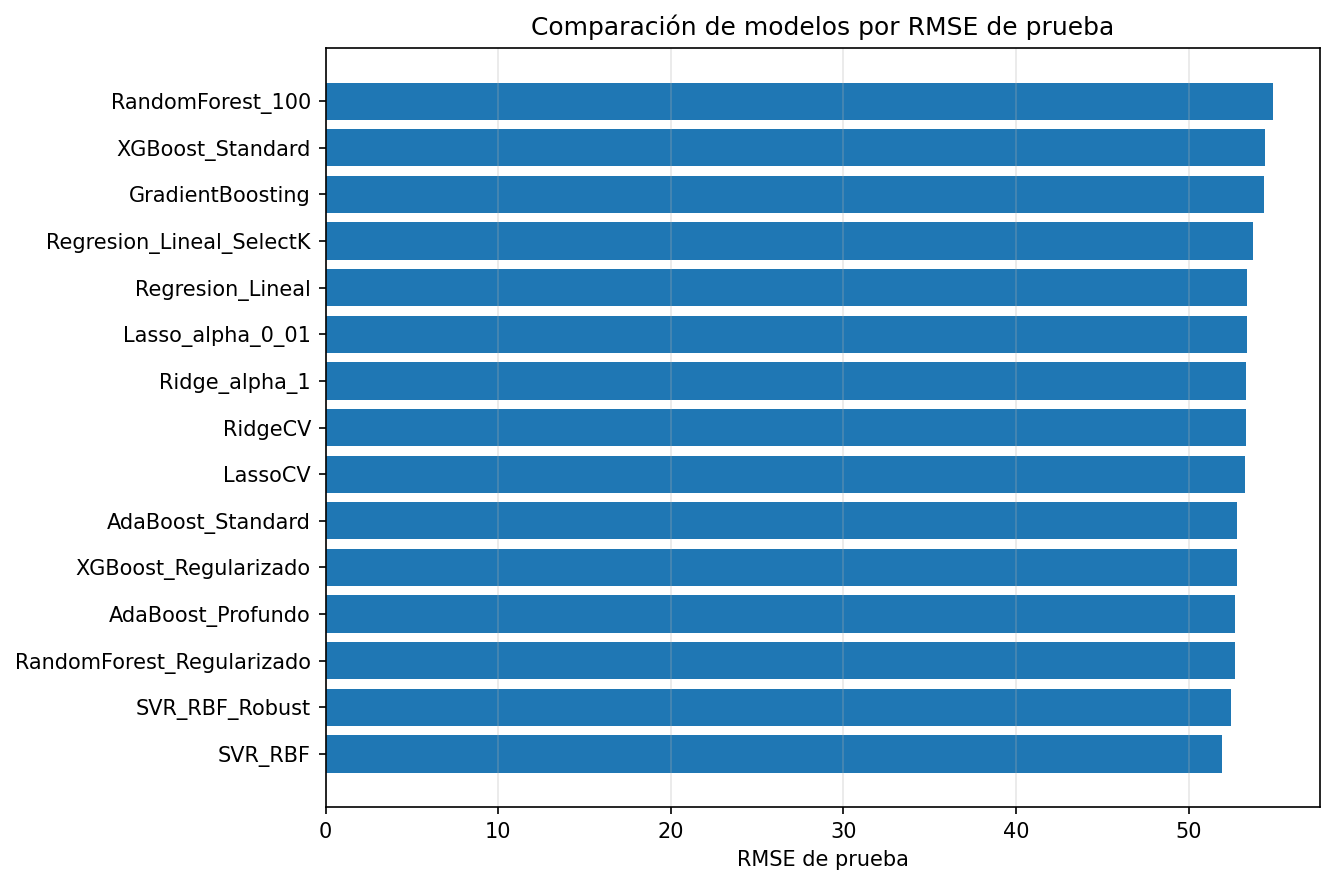
\includegraphics[width=0.9\textwidth]{benchmark_rmse.png}
\caption{Comparación de modelos por RMSE de prueba.}
\label{fig:benchmark_rmse}
\end{figure}

\begin{figure}[H]
\centering
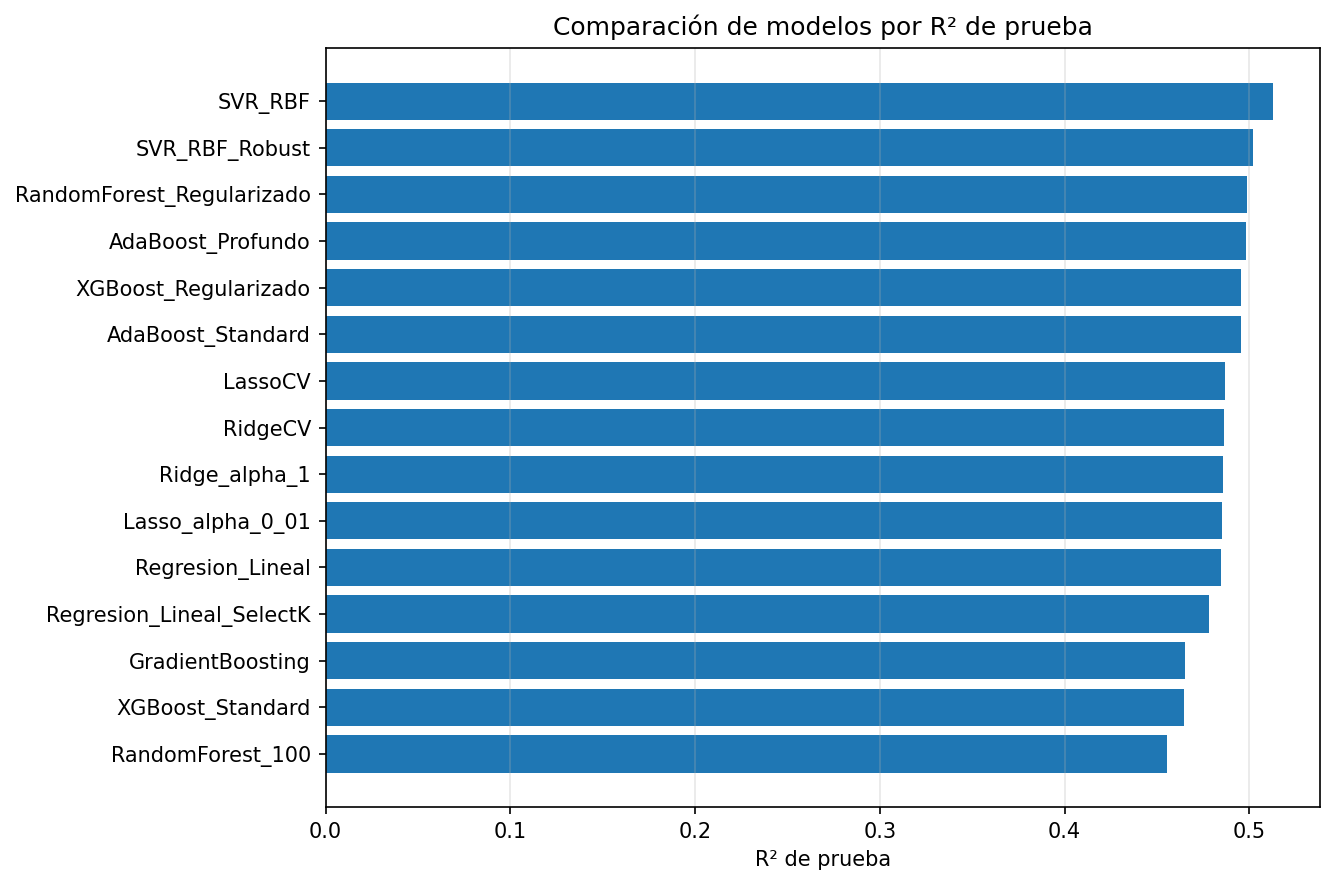
\includegraphics[width=0.9\textwidth]{benchmark_r2.png}
\caption{Comparación de modelos por $R^2$ de prueba.}
\label{fig:benchmark_r2}
\end{figure}

\begin{figure}[H]
\centering
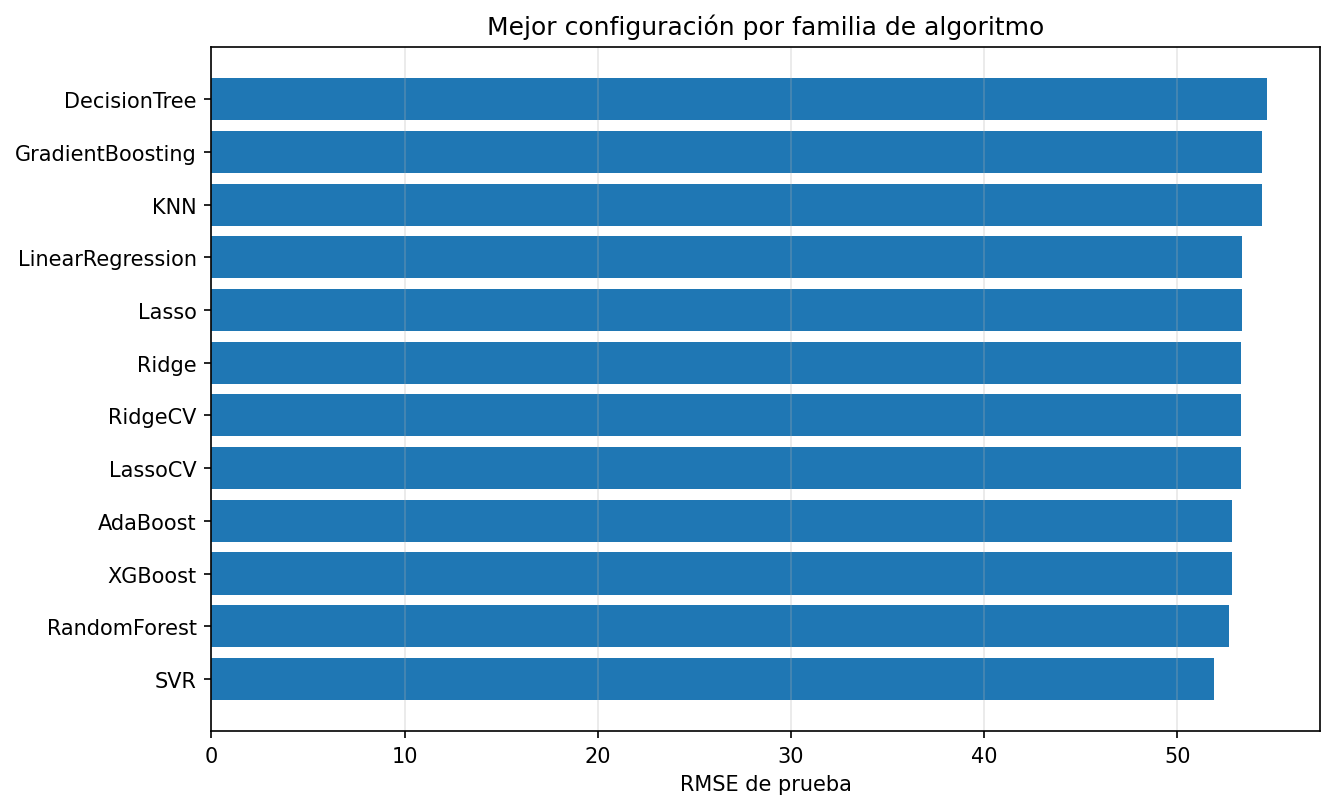
\includegraphics[width=0.9\textwidth]{benchmark_familias.png}
\caption{Mejor configuración por familia de algoritmo.}
\label{fig:fam}
\end{figure}

\subsection{Selección del mejor modelo}
De acuerdo con el criterio principal de selección, el mejor modelo fue \textbf{Regresión Lineal con escalamiento estándar}, con un RMSE promedio en validación cruzada de 55.6310 y un RMSE en prueba de 53.3696. Aunque algunos modelos no lineales obtuvieron un RMSE de prueba ligeramente menor, la regresión lineal fue más estable en validación cruzada.

\begin{table}[H]
\centering
\caption{Métricas del mejor modelo seleccionado.}
\begin{tabular}{lr}
\toprule
Métrica & Valor \\
\midrule
Test RMSE & 53.3696 \\
Test MAE & 41.5485 \\
Test $R^2$ & 0.4849 \\
Test MAPE & 37.3110\% \\
\bottomrule
\end{tabular}
\end{table}

\begin{figure}[H]
\centering
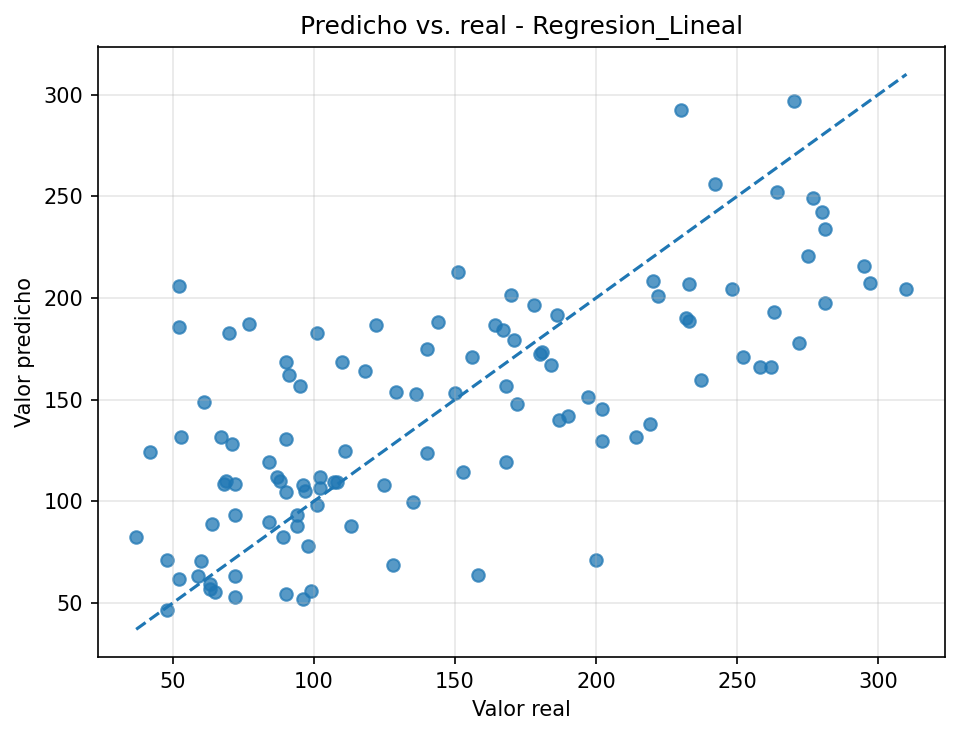
\includegraphics[width=0.75\textwidth]{predicho_vs_real_mejor.png}
\caption{Valores predichos contra valores reales del mejor modelo.}
\label{fig:pred_vs_real}
\end{figure}

\begin{figure}[H]
\centering
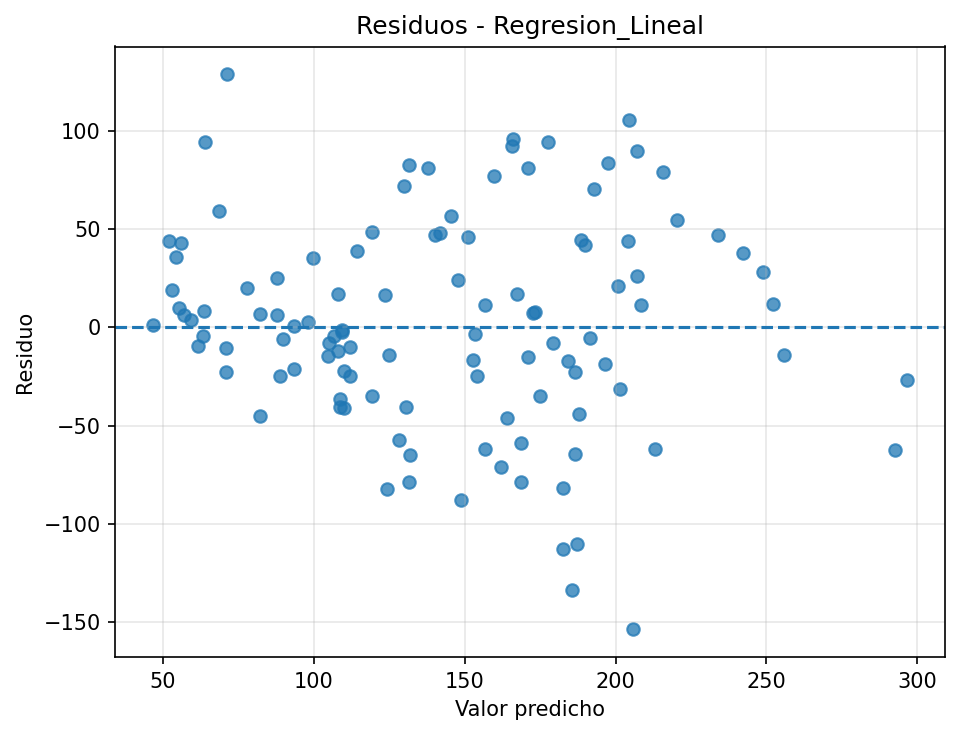
\includegraphics[width=0.75\textwidth]{residuos_mejor.png}
\caption{Análisis gráfico de residuos del mejor modelo.}
\label{fig:residuos}
\end{figure}

\subsection{Importancia e interpretación de variables}
Para el modelo lineal, la importancia se interpreta mediante la magnitud de los coeficientes. Las variables con mayor peso absoluto fueron \texttt{s1}, \texttt{s5}, \texttt{bmi}, \texttt{s2} y \texttt{bp}. La Figura \ref{fig:topvars} resume los coeficientes más relevantes.

\begin{figure}[H]
\centering
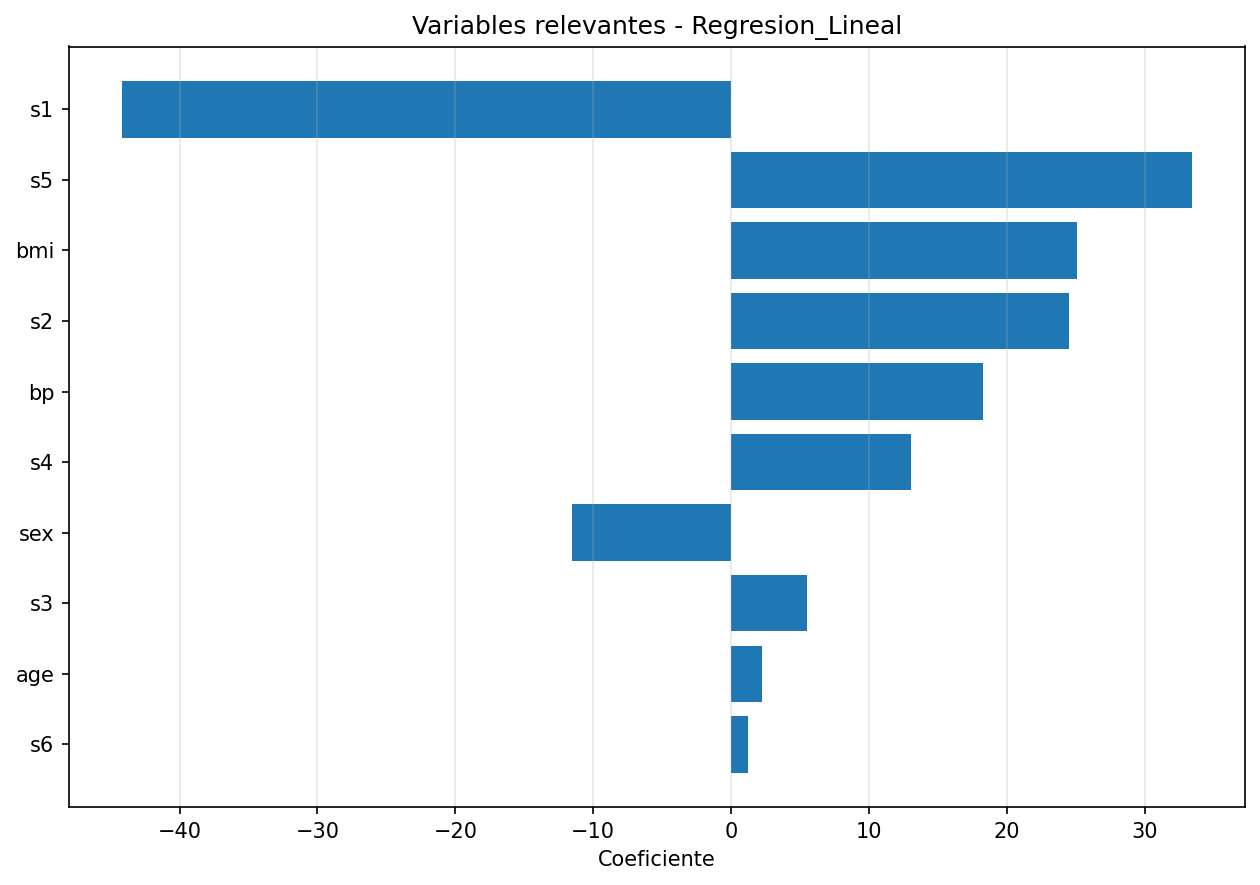
\includegraphics[width=0.85\textwidth]{top_variables_mejor.png}
\caption{Variables más relevantes del mejor modelo.}
\label{fig:topvars}
\end{figure}

\section{Comparación entre familias de algoritmos de regresión}

Esta sección aborda el inciso (d) del laboratorio: generar modelos de regresión pertenecientes a familias distintas y comparar su desempeño. A diferencia de la comparación intra-familia, donde se evalúan variaciones de hiperparámetros dentro de un mismo tipo de algoritmo, aquí el análisis se centra en las diferencias estructurales entre categorías de algoritmos.

\subsection{Familias de algoritmos evaluadas}

Los modelos se agruparon en cuatro familias, cada una con al menos dos configuraciones:

\begin{enumerate}
    \item \textbf{Familia lineal}: \texttt{LinearRegression}, \texttt{Ridge} ($\alpha=1$), \texttt{RidgeCV}, \texttt{Lasso} ($\alpha=0.01$), \texttt{LassoCV}. Estos modelos asumen una relación lineal entre predictores y variable objetivo. Ridge y Lasso agregan regularización $L_2$ y $L_1$ respectivamente para controlar la magnitud de los coeficientes y mitigar multicolinealidad.
    \item \textbf{Familia basada en kernels (SVM)}: \texttt{SVR} con kernels \texttt{rbf}, \texttt{linear} y \texttt{poly}. El kernel \texttt{rbf} permite modelar relaciones no lineales proyectando los datos a un espacio de mayor dimensión; \texttt{linear} produce un hiperplano similar a la regresión lineal pero con margen de tolerancia $\epsilon$; \texttt{poly} aplica transformaciones polinómicas.
    \item \textbf{Familia basada en árboles}: \texttt{DecisionTreeRegressor} en su versión estándar (sin restricción de profundidad) y con poda (\texttt{max\_depth=4}, \texttt{min\_samples\_split=10}, \texttt{min\_samples\_leaf=5}). Los árboles particionan recursivamente el espacio de predictores mediante reglas binarias.
    \item \textbf{Familia de ensambles}: \texttt{RandomForestRegressor} (100 y regularizado), \texttt{GradientBoostingRegressor} y \texttt{XGBoostRegressor}. Random Forest combina múltiples árboles mediante \textit{bagging}, mientras que Gradient Boosting y XGBoost construyen árboles secuenciales que corrigen los residuos del modelo previo (\textit{boosting}).
\end{enumerate}

\subsection{Configuración experimental}

Todos los modelos se evaluaron bajo las mismas condiciones:
\begin{itemize}
    \item Partición 75\% entrenamiento y 25\% prueba con semilla fija (\texttt{random\_state=42}).
    \item Escalamiento con \texttt{StandardScaler} aplicado antes del entrenamiento.
    \item Validación cruzada de 5 folds (\texttt{KFold}, \texttt{shuffle=True}).
    \item Métricas: MSE, RMSE, MAE y $R^2$, tanto en validación cruzada como en prueba.
\end{itemize}

\subsection{Benchmark general entre familias}

La Tabla~\ref{tab:cross_family_benchmark} resume el desempeño de todos los modelos evaluados, ordenados por RMSE de validación cruzada.

\begin{table}[H]
\centering
\caption{Benchmark comparativo entre familias de algoritmos de regresión.}
\label{tab:cross_family_benchmark}
\resizebox{\textwidth}{!}{%
\begin{tabular}{llrrrrrrr}
\toprule
Modelo & Familia & CV RMSE & CV $R^2$ & Test MSE & Test RMSE & Test MAE & Test $R^2$ \\
\midrule
Ridge ($\alpha$=1) & Lineal & 56.0688 & 0.4615 & 2842.83 & 53.3182 & 41.5073 & 0.4859 \\
Lasso ($\alpha$=0.01) & Lineal & 56.1111 & 0.4607 & 2847.18 & 53.3590 & 41.5418 & 0.4851 \\
LinearRegression & Lineal & 56.1186 & 0.4606 & 2848.31 & 53.3696 & 41.5485 & 0.4849 \\
LassoCV & Lineal & 56.2298 & 0.4581 & 2838.42 & 53.2768 & 41.4814 & 0.4867 \\
SVR (linear) & Kernel/SVM & 56.2500 & 0.4586 & 2964.29 & 54.4453 & 41.9288 & 0.4639 \\
RidgeCV & Lineal & 56.2677 & 0.4580 & 2841.64 & 53.3070 & 41.4962 & 0.4861 \\
XGBoost & Ensamble & 59.3126 & 0.3963 & 2959.32 & 54.3996 & 42.4433 & 0.4648 \\
RandomForest (reg) & Ensamble & 59.4079 & 0.3958 & 2771.66 & 52.6466 & 42.6534 & 0.4988 \\
GradientBoosting & Ensamble & 59.5407 & 0.3923 & 2919.76 & 54.0348 & 42.4841 & 0.4720 \\
SVR (rbf) & Kernel/SVM & 60.0342 & 0.3829 & 2762.12 & 52.5558 & 40.1235 & 0.5005 \\
RandomForest (100) & Ensamble & 61.0732 & 0.3588 & 3011.06 & 54.8732 & 43.7833 & 0.4555 \\
SVR (poly) & Kernel/SVM & 68.7519 & 0.1974 & 3943.43 & 62.7968 & 50.6663 & 0.2869 \\
DecisionTree (podado) & Árbol & 69.6626 & 0.1679 & 2986.50 & 54.6489 & 43.5694 & 0.4599 \\
DecisionTree (std) & Árbol & 78.1711 & $-$0.0591 & 5940.41 & 77.0740 & 58.7297 & $-$0.0743 \\
\bottomrule
\end{tabular}%
}
\end{table}

\begin{figure}[H]
\centering
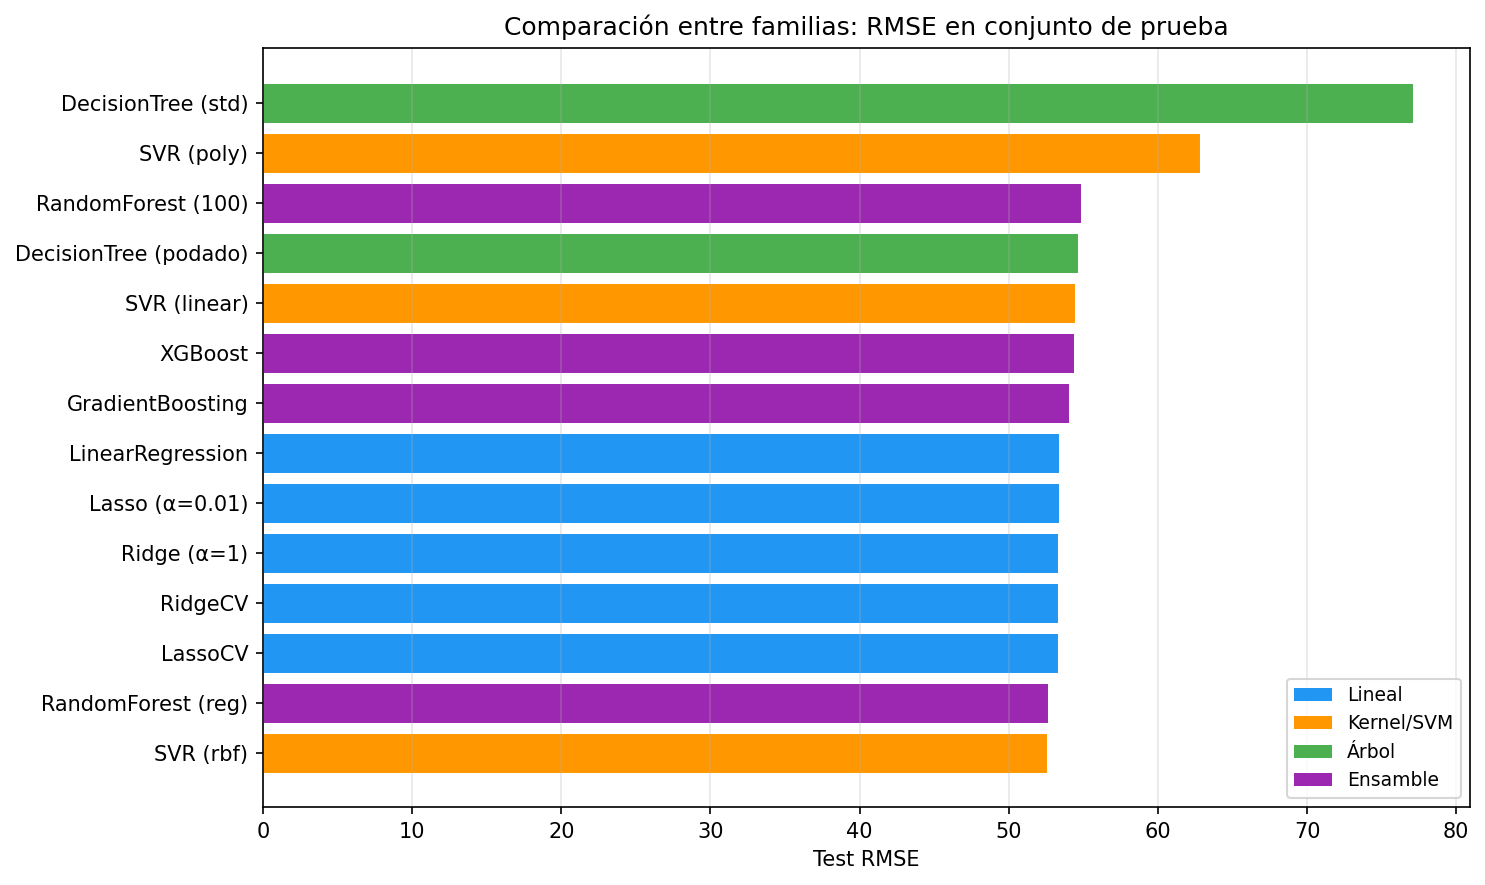
\includegraphics[width=0.92\textwidth]{cross_family_rmse.png}
\caption{Comparación entre familias: RMSE en conjunto de prueba. Los colores representan la familia del algoritmo.}
\label{fig:cf_rmse}
\end{figure}

\begin{figure}[H]
\centering
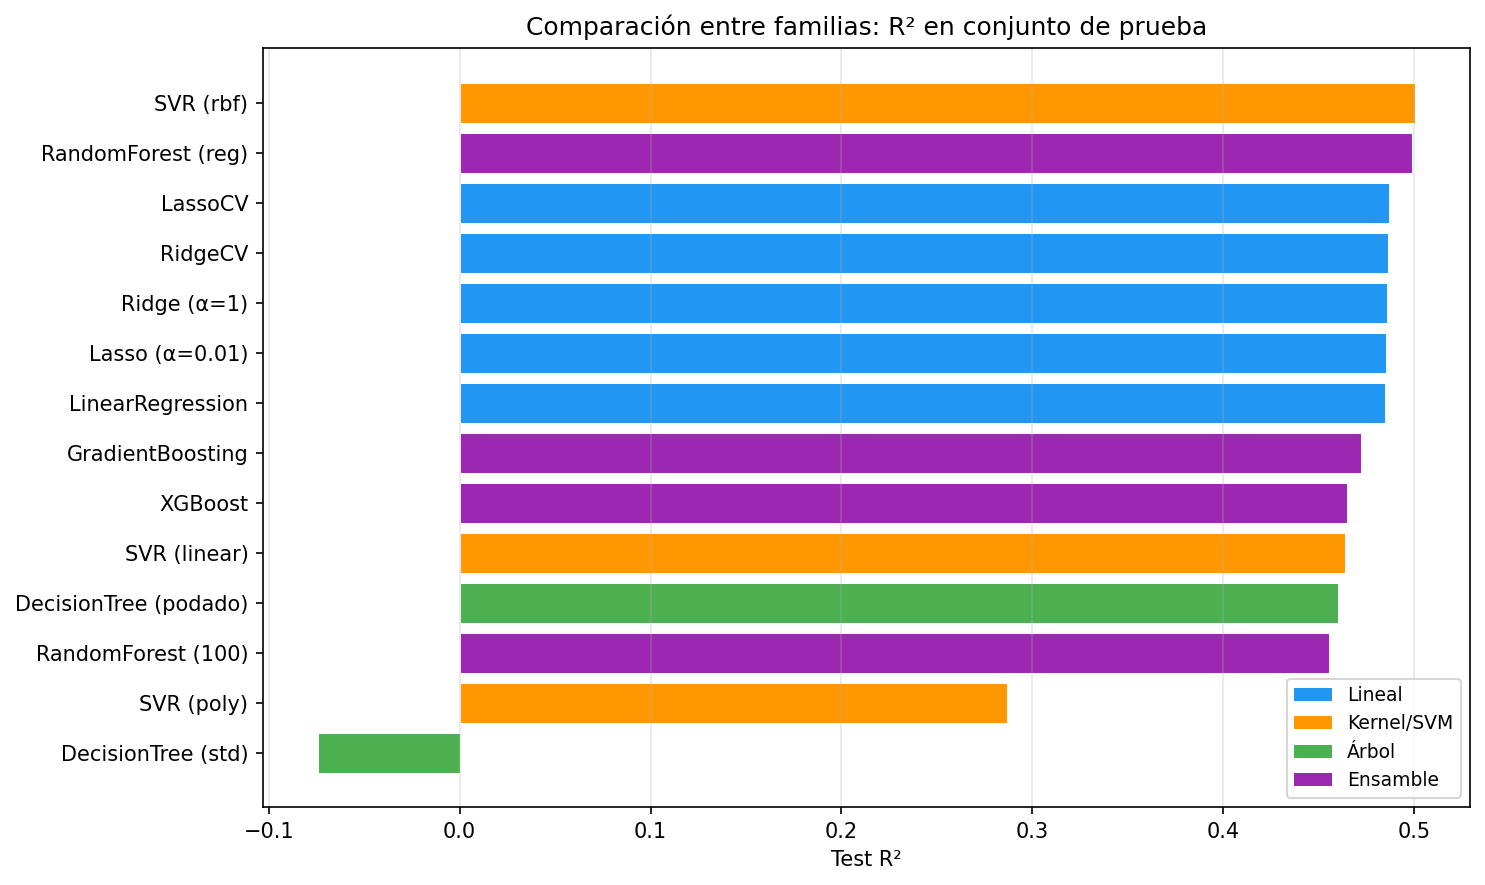
\includegraphics[width=0.92\textwidth]{cross_family_r2.png}
\caption{Comparación entre familias: $R^2$ en conjunto de prueba.}
\label{fig:cf_r2}
\end{figure}

\subsection{Mejor modelo por familia}

La Tabla~\ref{tab:best_per_family} presenta el mejor representante de cada familia según el RMSE promedio de validación cruzada.

\begin{table}[H]
\centering
\caption{Mejor modelo por familia de algoritmo.}
\label{tab:best_per_family}
\begin{tabular}{llrrrr}
\toprule
Familia & Mejor modelo & CV RMSE & Test RMSE & Test MAE & Test $R^2$ \\
\midrule
Lineal & Ridge ($\alpha$=1) & 56.0688 & 53.3182 & 41.5073 & 0.4859 \\
Kernel/SVM & SVR (linear) & 56.2500 & 54.4453 & 41.9288 & 0.4639 \\
Ensamble & XGBoost & 59.3126 & 54.3996 & 42.4433 & 0.4648 \\
Árbol & DT (podado) & 69.6626 & 54.6489 & 43.5694 & 0.4599 \\
\bottomrule
\end{tabular}
\end{table}

\begin{figure}[H]
\centering
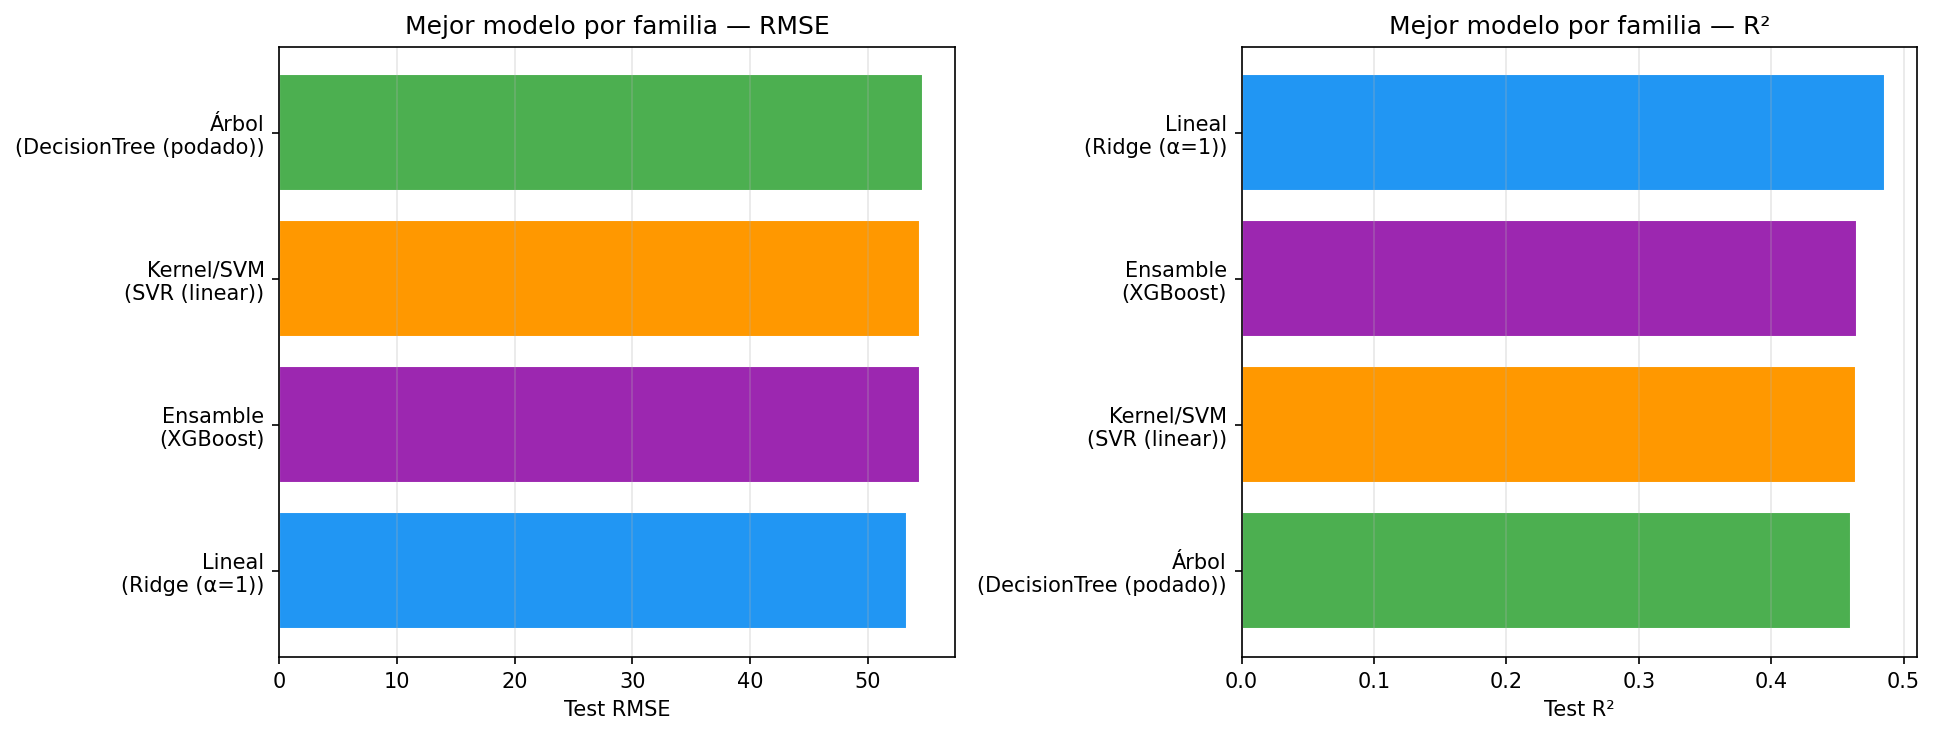
\includegraphics[width=0.95\textwidth]{best_per_family.png}
\caption{Mejor configuración por familia de algoritmo: RMSE y $R^2$ en prueba.}
\label{fig:best_fam}
\end{figure}

\subsection{Estabilidad: validación cruzada frente a prueba}

La Figura~\ref{fig:cv_vs_test} permite identificar modelos con sobreajuste (puntos alejados de la diagonal) y modelos estables (puntos cercanos a ella).

\begin{figure}[H]
\centering
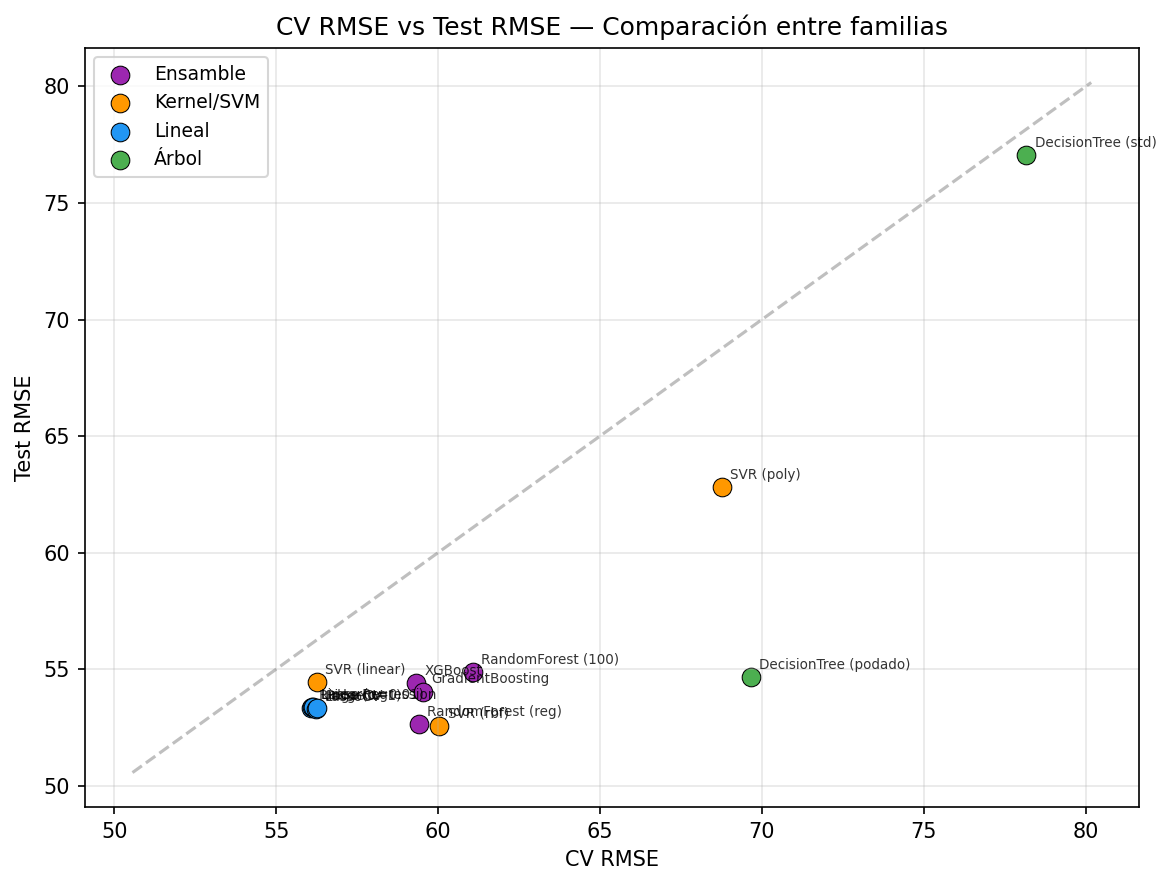
\includegraphics[width=0.85\textwidth]{cv_vs_test_rmse.png}
\caption{RMSE en validación cruzada frente a RMSE en prueba. Los puntos cercanos a la diagonal indican modelos estables.}
\label{fig:cv_vs_test}
\end{figure}

\begin{figure}[H]
\centering
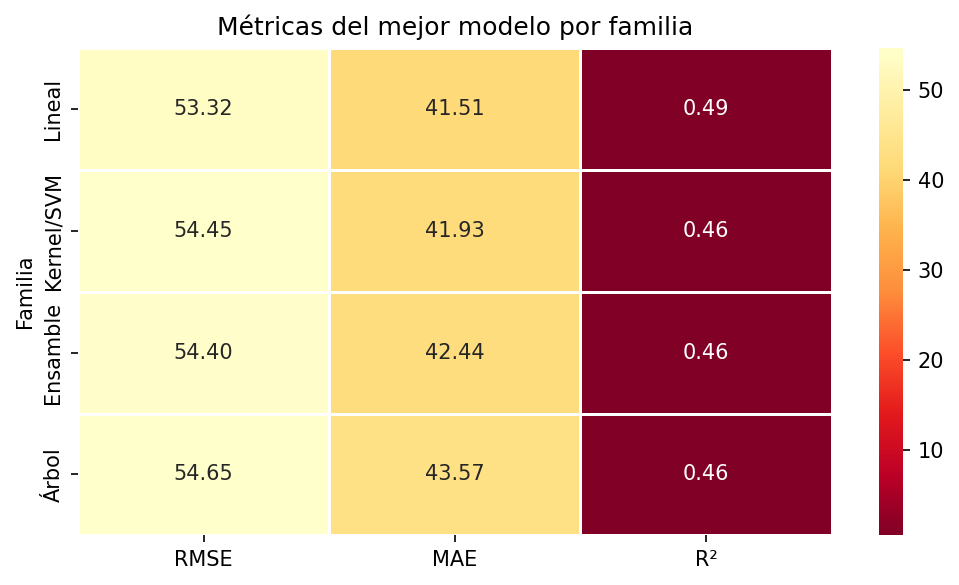
\includegraphics[width=0.7\textwidth]{heatmap_families.png}
\caption{Heatmap de métricas del mejor modelo por familia.}
\label{fig:heatmap_fam}
\end{figure}

\subsection{Análisis del mejor modelo global}

El modelo seleccionado como mejor configuración global fue \textbf{Ridge ($\alpha$=1)}, perteneciente a la familia lineal, con un CV RMSE de 56.0688 y un Test RMSE de 53.3182. Sus métricas completas en el conjunto de prueba fueron:

\begin{table}[H]
\centering
\caption{Métricas del mejor modelo global: Ridge ($\alpha$=1).}
\begin{tabular}{lr}
\toprule
Métrica & Valor \\
\midrule
Test MSE & 2842.83 \\
Test RMSE & 53.3182 \\
Test MAE & 41.5073 \\
Test $R^2$ & 0.4859 \\
\bottomrule
\end{tabular}
\end{table}

\begin{figure}[H]
\centering
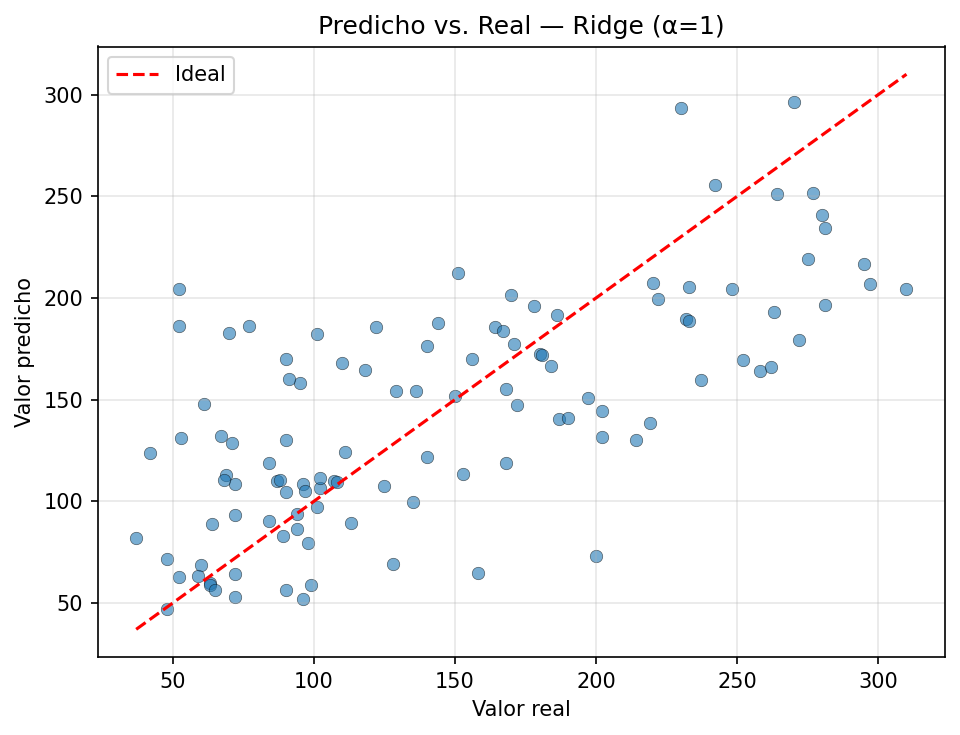
\includegraphics[width=0.72\textwidth]{pred_vs_real_best.png}
\caption{Valores predichos contra valores reales del modelo Ridge ($\alpha$=1).}
\label{fig:pred_real_best}
\end{figure}

\begin{figure}[H]
\centering
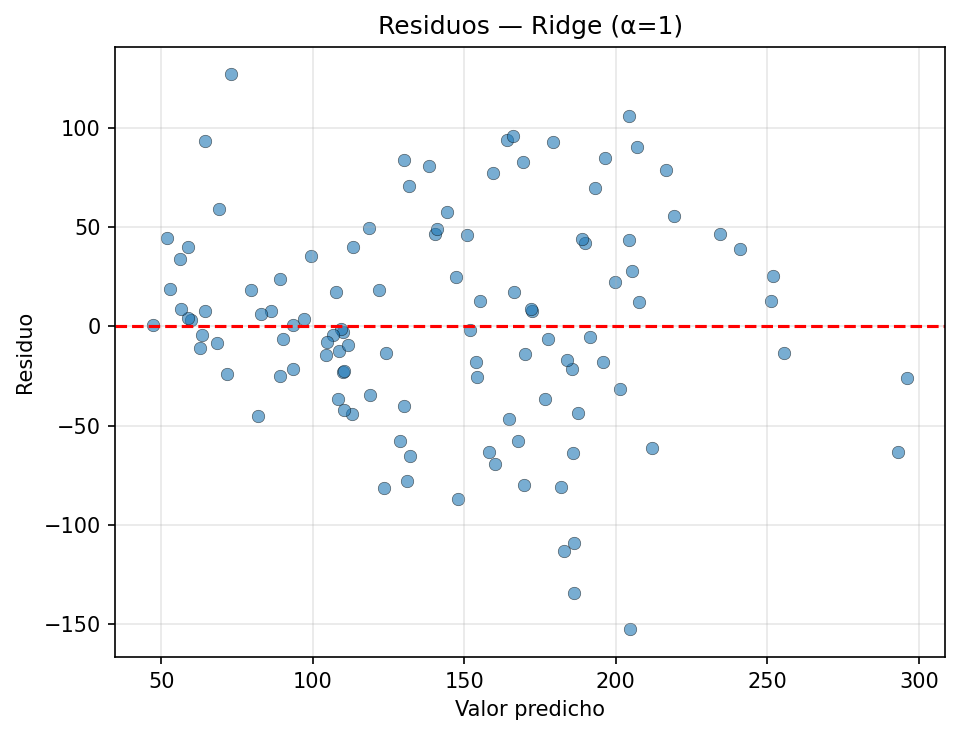
\includegraphics[width=0.72\textwidth]{residuos_best.png}
\caption{Análisis gráfico de residuos del modelo Ridge ($\alpha$=1).}
\label{fig:resid_best}
\end{figure}

\subsection{Discusión entre familias}

\subsubsection{Familia lineal}
Los modelos lineales dominaron la comparación en validación cruzada. Ridge, Lasso y LinearRegression obtuvieron CV RMSE en el rango 56.07--56.27, con Test $R^2$ alrededor de 0.485. Esto indica que la relación entre predictores y variable objetivo en el dataset Diabetes tiene un componente fundamentalmente lineal. La regularización $L_2$ de Ridge ofreció una ligera ventaja por su capacidad de reducir la varianza de los coeficientes ante predictores correlacionados.

\subsubsection{Familia basada en kernels (SVM)}
SVR con kernel lineal se comportó de forma similar a los modelos lineales (CV RMSE 56.25), lo cual es consistente: un kernel lineal es esencialmente una regresión con margen. SVR con kernel RBF obtuvo el \textbf{mejor Test RMSE absoluto} (52.56), pero su CV RMSE fue mayor (60.03), lo que señala menor estabilidad y posible sobreajuste a la partición de prueba. SVR polinómico fue claramente inferior, lo que sugiere que la transformación cúbica no se adapta a la estructura de estos datos.

\subsubsection{Familia basada en árboles}
El árbol sin restricciones presentó sobreajuste severo: CV $R^2$ negativo ($-$0.06) y Test $R^2$ de $-$0.07, indicando un modelo que generaliza peor que la media. La versión podada mejoró drásticamente (Test $R^2$=0.46), confirmando que la regulación mediante \texttt{max\_depth} y \texttt{min\_samples\_leaf} es indispensable. No obstante, un solo árbol no captura suficiente información para competir con los modelos lineales en este dataset.

\subsubsection{Familia de ensambles}
RandomForest regularizado y XGBoost obtuvieron resultados competitivos en prueba (Test $R^2$ de 0.4988 y 0.4648 respectivamente), pero sus CV RMSE fueron superiores a los lineales ($\sim$59). Esto indica que los ensambles capturan relaciones no lineales parciales, pero en un dataset con estructura predominantemente lineal y solo 442 observaciones, la complejidad adicional no se traduce en una ventaja consistente. Es notable que RandomForest regularizado alcanzó un Test $R^2$ cercano a 0.50, sugiriendo que con datasets más grandes o de estructura más compleja podría superar a los modelos lineales.

\subsection{Ventajas y limitaciones por familia}

\begin{table}[H]
\centering
\caption{Ventajas y limitaciones de cada familia en el contexto del dataset Diabetes.}
\resizebox{\textwidth}{!}{%
\begin{tabular}{lp{6.5cm}p{6.5cm}}
\toprule
Familia & Ventajas & Limitaciones \\
\midrule
Lineal & Mejor estabilidad en CV, interpretabilidad directa mediante coeficientes, bajo costo computacional. & Asume linealidad; no captura interacciones ni relaciones no lineales. \\
Kernel/SVM & SVR RBF logra el menor error puntual en prueba; flexibilidad con distintos kernels. & Sensible a hiperparámetros ($C$, $\epsilon$, $\gamma$), menor estabilidad en CV, requiere escalamiento obligatorio. \\
Árbol & Interpretabilidad mediante reglas, manejo natural de no linealidad. & Alto riesgo de sobreajuste sin poda; peor desempeño entre todas las familias. \\
Ensamble & Captura relaciones no lineales, reduce varianza respecto a un árbol individual. & Mayor costo computacional, CV RMSE superior al lineal en este dataset, riesgo de sobreajuste con demasiados estimadores. \\
\bottomrule
\end{tabular}%
}
\end{table}

\subsection{Conclusión de la comparación entre familias}

La comparación entre familias de algoritmos sobre el dataset Diabetes revela que los modelos lineales, particularmente Ridge con regularización $L_2$, representan la mejor opción global al equilibrar estabilidad en validación cruzada, bajo error en prueba e interpretabilidad. Los ensambles y SVR con kernel RBF mostraron capacidad para capturar señales no lineales residuales, pero sin una ventaja consistente bajo validación cruzada. Los árboles de decisión individuales resultaron la familia menos adecuada para este problema.

El criterio de selección prioriza la robustez medida por CV RMSE, dado que el desempeño en una única partición de prueba puede estar sujeto a variabilidad muestral. Bajo este criterio, \textbf{Ridge ($\alpha$=1)} fue el modelo seleccionado como mejor representante global.

\section{Análisis de resultados}

\subsection{Modelos lineales y penalizados}
La regresión lineal, Ridge y Lasso presentaron resultados muy similares. Esto indica que el dataset tiene una estructura aproximadamente lineal y que la penalización no produjo cambios drásticos. Ridge y Lasso reducen la complejidad de los coeficientes, pero en este caso la regresión lineal simple mantuvo el mejor promedio de validación cruzada.

\subsection{KNN y SVR}
KNN presentó un desempeño inferior al de los modelos lineales, lo cual puede explicarse por la dificultad de estimar valores continuos mediante promedios locales cuando la estructura global tiene un componente lineal importante. SVR obtuvo un buen $R^2$ en prueba, pero su RMSE de validación cruzada fue mayor, por lo que se considera menos estable bajo el criterio de selección definido.

\subsection{Árboles, Random Forest y Boosting}
El árbol de regresión sin restricciones mostró evidencia de sobreajuste. La versión podada mejoró su desempeño, aunque no superó a los modelos lineales. Random Forest y XGBoost regularizado obtuvieron resultados competitivos en prueba, pero su error promedio de validación cruzada fue mayor. Esto sugiere que los ensambles capturan relaciones no lineales, pero no necesariamente generalizan mejor en este dataset específico.

\section{Conclusiones}
\begin{enumerate}
    \item El dataset Diabetes es adecuado para regresión porque su variable objetivo es cuantitativa y continua.
    \item La regresión lineal con escalamiento estándar fue seleccionada como mejor modelo por presentar el menor RMSE promedio en validación cruzada.
    \item Ridge y Lasso obtuvieron resultados casi equivalentes, lo que confirma que la regularización no fue determinante en este conjunto de datos.
    \item Los modelos basados en árboles y ensambles requieren control de complejidad para evitar sobreajuste.
    \item SVR y Random Forest lograron métricas competitivas en prueba, pero no superaron la estabilidad de los modelos lineales bajo validación cruzada.
    \item El análisis de residuos y la comparación entre predicción y valor real son indispensables para complementar las métricas numéricas.
\end{enumerate}

\section{Trabajo reproducible}
El laboratorio se entrega junto con los siguientes archivos:
\begin{itemize}
    \item \texttt{ModuloRegresionLab03.py}: paquete pythónico con clases de análisis y experimentación.
    \item \texttt{InterfazRegresionLab03.ipynb}: notebook de ejecución paso a paso.
    \item \texttt{main\_lab3\_regresion.tex}: documento LaTeX del informe.
    \item \texttt{diabetes\_regression\_lab03.csv}: dataset reproducible usado en el experimento base.
    \item \texttt{outputs\_lab03/}: carpeta con gráficos y resultados generados.
\end{itemize}

\begin{thebibliography}{9}
\bibitem{hastie}
Hastie, T., Tibshirani, R., \& Friedman, J. (2009). \textit{The Elements of Statistical Learning}. Springer.

\bibitem{james}
James, G., Witten, D., Hastie, T., \& Tibshirani, R. (2021). \textit{An Introduction to Statistical Learning}. Springer.

\bibitem{breiman}
Breiman, L. (2001). Random Forests. \textit{Machine Learning}, 45, 5--32.

\bibitem{friedman}
Friedman, J. H. (2001). Greedy function approximation: A gradient boosting machine. \textit{Annals of Statistics}, 29(5), 1189--1232.

\bibitem{chen}
Chen, T., \& Guestrin, C. (2016). XGBoost: A scalable tree boosting system. \textit{Proceedings of the 22nd ACM SIGKDD International Conference on Knowledge Discovery and Data Mining}.
\end{thebibliography}

\end{document}
